\documentclass[conference]{IEEEtran}
\IEEEoverridecommandlockouts
\usepackage[T1]{fontenc}
\usepackage{mathptmx}
\usepackage{cite}
\usepackage{amsmath,amssymb}
\usepackage{graphicx}
\usepackage{booktabs}
\usepackage{array}
\usepackage{xcolor}
\usepackage{tikz}
\usetikzlibrary{arrows.meta,positioning,fit,calc,shapes.geometric}
\usepackage[hidelinks]{hyperref}
\usepackage{listings}
\lstset{basicstyle=\ttfamily\footnotesize,columns=fullflexible,frame=single,
        framerule=0.3pt,xleftmargin=2pt,xrightmargin=2pt}

\definecolor{stIF}{HTML}{DCEBFA}
\definecolor{stID}{HTML}{E3F2DC}
\definecolor{stEX}{HTML}{FCE9D4}
\definecolor{stMEM}{HTML}{EDE3F6}
\definecolor{stWB}{HTML}{F9DCDC}
\definecolor{hz}{HTML}{FFF4C2}

\begin{document}

\title{Design and Verification of a 5-Stage Pipelined RISC-V (RV32I) Processor in Verilog HDL}

\author{
\IEEEauthorblockN{Abhishek Kumar Patel}
\and
\IEEEauthorblockN{Yogesh Modi}
\and
\IEEEauthorblockN{Kapish Rohilla}
\and
\IEEEauthorblockN{Vikash Kumar}
\and
\IEEEauthorblockN{Prateek Shakya}
}

\maketitle

% ---------------------------------------------------------------------------
\begin{abstract}
This paper presents the design, implementation and functional verification of a
32-bit, five-stage pipelined processor for a subset of the RISC-V RV32I base integer
instruction set. The processor is written in synthesizable-style Verilog HDL and is
organised into the classic Instruction Fetch (IF), Instruction Decode (ID), Execute (EX),
Memory (MEM) and Write-Back (WB) stages, separated by four pipeline registers. It supports
29 instructions covering register and immediate arithmetic, logical and shift operations,
word loads and stores, conditional branches, jumps and upper-immediate loads. Data hazards
are resolved by a forwarding unit that bypasses results from the EX/MEM and MEM/WB
registers to the ALU, a hazard detection unit that inserts a single-cycle bubble for
load-use dependencies, and a write-first register file. Control hazards are handled by
resolving branches and jumps in the EX stage under a predict-not-taken policy, flushing
two wrongly fetched instructions on a taken transfer. Structural hazards are avoided by
separate instruction and data memories. The design was verified with Icarus Verilog using
16 self-checking unit testbenches (204 checks) and six system-level assembly programs
(36 architectural-state checks), all of which pass. A testbench performance counter
measures cycles per instruction (CPI) on every program; including pipeline fill, the
measured CPI ranges from 1.19 to 2.09, and every cycle count matches the analytical
model $N + 4 + S + 2T$ for $N$ instructions, $S$ load-use stalls and $T$ taken branches
or jumps.
\end{abstract}

\begin{IEEEkeywords}
RISC-V, RV32I, pipelined processor, Verilog HDL, data forwarding, hazard detection,
computer architecture, functional verification
\end{IEEEkeywords}

% ---------------------------------------------------------------------------
\section{Introduction}
A single-cycle processor completes every instruction in one long clock cycle, so the clock
period is set by the slowest instruction. Pipelining divides instruction execution into
stages and overlaps the stages of consecutive instructions, in the same way as an assembly
line. In the ideal case one instruction completes every cycle, and the clock period is set
by the slowest \emph{stage} rather than the slowest instruction~\cite{pattersonRV,hennessyQA}.

Overlapping instructions introduces \emph{hazards}: an instruction may need a result that
has not yet been written back (data hazard), the next instruction address may not yet be
known (control hazard), or two stages may need the same resource (structural hazard).
A correct pipelined processor must detect and resolve all three.

RISC-V is an open, royalty-free instruction set architecture developed at the University
of California, Berkeley~\cite{rvmanual,asanovic2014free}. Its regular, fixed-length
32-bit encoding and small base integer set make it well suited to teaching and to
hardware design projects. This project implements an RV32I subset on a five-stage
pipeline with full forwarding and hazard handling, and verifies it in simulation.

The main contributions of this work are:
\begin{itemize}
  \item a modular Verilog implementation of a five-stage RV32I pipeline whose modules
        share one header of opcodes and control codes;
  \item forwarding, load-use stall and branch-flush logic that together resolve all
        data and control hazards for the supported instructions;
  \item a self-checking verification suite of unit testbenches and assembly programs,
        run by a single script.
\end{itemize}

Section~II reviews related work. Section~III describes the proposed design.
Section~IV reports verification and performance results, and Section~V lists
individual contributions.

% ---------------------------------------------------------------------------
\section{Literature Review}

\subsection{RISC Philosophy and Classic Pipelines}
Patterson and Ditzel argued that a reduced instruction set with simple, uniform
instructions allows a simpler and faster implementation than complex instruction
sets~\cite{patterson1980risc}. The Stanford MIPS project demonstrated a pipelined
RISC microprocessor in which the compiler and hardware cooperate to keep the pipeline
busy~\cite{hennessy1982mips}. The five-stage IF--ID--EX--MEM--WB organisation used in
this project is the classic pipeline described by Hennessy and Patterson, which remains
the standard teaching model for pipelined datapaths~\cite{hennessyQA,pattersonRV}.

\subsection{Hazard Resolution Techniques}
Data hazards can be handled by stalling until the producer writes the register file,
but this wastes cycles for every dependent pair. \emph{Forwarding} (bypassing) instead
routes a result from a later pipeline register directly to the ALU input, so most
read-after-write dependencies cost no cycles~\cite{pattersonRV}. A load followed
immediately by a dependent instruction still needs one stall cycle, because the loaded
value is available only at the end of MEM. Control hazards are commonly handled by
predicting the branch outcome; the simplest static scheme predicts not-taken and
flushes the wrongly fetched instructions when the branch is taken~\cite{hennessyQA}.
Dynamic scheduling, as in Tomasulo's algorithm~\cite{tomasulo1967}, removes more stalls
but at a much higher hardware cost and is outside the scope of an in-order design.

\subsection{The RISC-V ISA and Open Implementations}
The RISC-V specification defines a small base integer ISA (RV32I/RV64I) with optional
standard extensions~\cite{rvmanual,waterman2011}. Asanovi\'c and Patterson made the case
for a free and open ISA usable by academia and industry alike~\cite{asanovic2014free}.
Open implementations span a wide range: the Rocket Chip generator produces an in-order
five-stage core~\cite{rocket2016}, while BOOM is a superscalar out-of-order
core~\cite{boom2015}. Harris and Harris present single-cycle, multicycle and pipelined
RISC-V microarchitectures in HDL as a teaching reference~\cite{harrisRV}.

\subsection{Reference Project}
We studied the open-source \emph{protocolx-riscv-pipelined-processor}
project~\cite{protocolx}, which implements a pipelined RISC-V processor in Verilog. It
helped us plan the module breakdown and test approach. All code in our repository was
written independently by the team.

\subsection{Gap Addressed}
Production cores are too large to study line by line, while textbook datapaths are
often given only as diagrams. This project fills the gap between them: a small, fully
documented and fully tested five-stage design in which each hazard mechanism is an
isolated, unit-tested module.

% ---------------------------------------------------------------------------
\section{Proposed Solution}

\subsection{Design Overview}
Fig.~\ref{fig:datapath} shows the processor. It is a Harvard machine: instruction memory
and data memory are separate 1024-word arrays, indexed by \texttt{addr[11:2]}, with
combinational reads. All registers update on the rising clock edge and use a
synchronous, active-high reset. The supported subset is listed in Table~\ref{tab:isa}.

\begin{table}[!t]
\centering
\caption{Supported RV32I Instruction Subset (29 Instructions)}
\label{tab:isa}
\renewcommand{\arraystretch}{1.1}
\begin{tabular}{@{}p{1.5cm}p{6.2cm}@{}}
\toprule
\textbf{Type} & \textbf{Instructions} \\ \midrule
R-type   & ADD, SUB, AND, OR, XOR, SLL, SRL, SRA, SLT, SLTU \\
I-type   & ADDI, ANDI, ORI, XORI, SLTI, SLTIU, SLLI, SRLI, SRAI \\
Load/Store & LW, SW (word-aligned) \\
Branch   & BEQ, BNE, BLT, BGE \\
Jump     & JAL, JALR \\
U-type   & LUI \\ \bottomrule
\end{tabular}
\end{table}

% ---------------- Datapath figure ----------------
\begin{figure*}[!t]
\centering
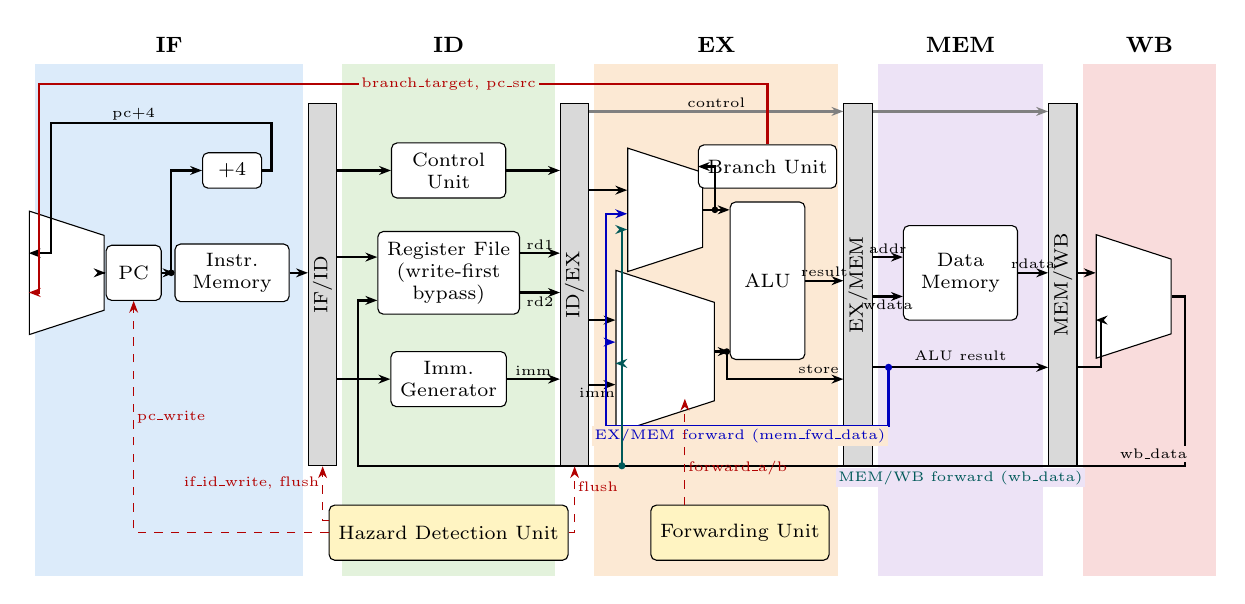
\begin{tikzpicture}[
  font=\scriptsize, >={Stealth[length=1.5mm]},
  blk/.style={draw, rounded corners=2pt, minimum width=1.45cm, minimum height=0.7cm, align=center, fill=white},
  preg/.style={draw, fill=gray!30, minimum width=0.36cm, minimum height=4.6cm},
  mux/.style={draw, fill=white, trapezium, trapezium angle=72, shape border rotate=270, minimum height=0.95cm, inner sep=1pt},
  w/.style={->, thick},
  ctl/.style={->, dashed, red!70!black},
  fA/.style={->, thick, blue!75!black},
  fB/.style={->, thick, teal!70!black},
  lbl/.style={font=\tiny, inner sep=1pt}
]
% stage backgrounds
\fill[stIF]  (-0.65,-3.85) rectangle (2.75,2.65);
\fill[stID]  (3.25,-3.85) rectangle (5.95,2.65);
\fill[stEX]  (6.45,-3.85) rectangle (9.55,2.65);
\fill[stMEM] (10.05,-3.85) rectangle (12.15,2.65);
\fill[stWB]  (12.65,-3.85) rectangle (14.35,2.65);
\foreach \x/\t in {1.05/IF, 4.6/ID, 8.0/EX, 11.1/MEM, 13.5/WB}
  \node[font=\footnotesize\bfseries] at (\x,2.9) {\t};
% pipeline registers
\node[preg] (r1) at (3.0,-0.15)  {}; \node[rotate=90] at (3.0,-0.15) {IF/ID};
\node[preg] (r2) at (6.2,-0.15)  {}; \node[rotate=90] at (6.2,-0.15) {ID/EX};
\node[preg] (r3) at (9.8,-0.15)  {}; \node[rotate=90] at (9.8,-0.15) {EX/MEM};
\node[preg] (r4) at (12.4,-0.15) {}; \node[rotate=90] at (12.4,-0.15) {MEM/WB};
% IF
\node[mux] (pcm) at (-0.25,0) {};
\node[blk, minimum width=0.7cm] (pc) at (0.6,0) {PC};
\node[blk] (im) at (1.85,0) {Instr.\\Memory};
\node[blk, minimum width=0.75cm, minimum height=0.45cm] (p4) at (1.85,1.3) {+4};
\draw[w] (pcm.east) -- (pc.west);
\draw[w] (pc.east) -- (im.west);
\draw[w] (pc.east) ++(0.12,0) |- (p4.west);
\fill (pc.east) ++(0.12,0) circle (1.2pt);
\draw[w] (p4.east) -- (2.35,1.3) -- (2.35,1.9) -- (-0.45,1.9) -- (-0.45,0.25) -- ($(pcm.west)+(0,0.25)$);
\node[lbl] at (0.6,2.02) {pc+4};
\draw[w] (im.east) -- (r1.west |- im.east);
% ID
\node[blk] (cu) at (4.6,1.3) {Control\\Unit};
\node[blk, minimum height=1.05cm] (rf) at (4.6,0) {Register File\\(write-first\\bypass)};
\node[blk] (ig) at (4.6,-1.35) {Imm.\\Generator};
\draw[w] (r1.east |- cu.west) -- (cu.west);
\draw[w] (r1.east |- 0,0.2) -- (rf.west |- 0,0.2);
\draw[w] (r1.east |- ig.west) -- (ig.west);
\draw[w] (cu.east) -- (r2.west |- cu.east);
\draw[w] ($(rf.east)+(0,0.25)$) -- node[lbl,above]{rd1} (r2.west |- 0,0.25);
\draw[w] ($(rf.east)+(0,-0.25)$) -- node[lbl,below]{rd2} (r2.west |- 0,-0.25);
\draw[w] (ig.east) -- node[lbl,above]{imm} (r2.west |- ig.east);
% control pass-through
\draw[w, gray] (r2.east |- 0,2.05) -- node[lbl,above,text=black]{control} (r3.west |- 0,2.05);
\draw[w, gray] (r3.east |- 0,2.05) -- (r4.west |- 0,2.05);
% EX
\node[mux] (ma) at (7.35,0.8) {};
\node[mux, minimum height=1.25cm] (mb) at (7.35,-1.0) {};
\node[blk, minimum width=0.95cm, minimum height=2.0cm] (alu) at (8.65,-0.1) {ALU};
\node[blk, minimum width=1.25cm, minimum height=0.55cm] (bu) at (8.65,1.35) {Branch Unit};
\draw[w] (r2.east |- 0,1.05) -- (ma.west |- 0,1.05);
\draw[w] (r2.east |- 0,-0.6) -- (mb.west |- 0,-0.6);
\draw[w] (ma.east) -- (alu.west |- ma.east);
\draw[w] (mb.east) -- (alu.west |- mb.east);
\draw[w] (r2.east |- 0,-1.42) -- node[lbl,below,pos=0.3]{imm} (mb.west |- 0,-1.42);
\draw[w] (ma.east) ++(0.15,0) |- (bu.west);
\fill (ma.east) ++(0.15,0) circle (1.2pt);
\draw[w] (alu.east) -- node[lbl,above]{result} (r3.west |- alu.east);
\draw[w] (mb.east) ++(0.15,0) -- ++(0,-0.35) -- (r3.west |- 0,-1.35);
\fill (mb.east) ++(0.15,0) circle (1.2pt);
\node[lbl] at (9.3,-1.22) {store};
% MEM
\node[blk, minimum height=1.2cm] (dm) at (11.1,0) {Data\\Memory};
\draw[w] (r3.east |- 0,0.2) -- node[lbl,above]{addr} (dm.west |- 0,0.2);
\draw[w] (r3.east |- 0,-0.3) -- node[lbl,below]{wdata} (dm.west |- 0,-0.3);
\draw[w] (dm.east) -- node[lbl,above]{rdata} (r4.west |- dm.east);
\draw[w] (r3.east |- 0,-1.2) -- (r4.west |- 0,-1.2);
\node[lbl] at (11.1,-1.05) {ALU result};
% WB
\node[mux] (wm) at (13.3,-0.3) {};
\draw[w] (r4.east |- 0,0) -- (wm.west |- 0,0);
\draw[w] (r4.east |- 0,-1.2) -- ++(0.3,0) |- (wm.west |- 0,-0.6);
% write-back path
\draw[w] (wm.east) -- (13.95,-0.3) -- (13.95,-2.45) -- (3.45,-2.45) -- (3.45,-0.35) -- (rf.west |- 0,-0.35);
\node[lbl, fill=stWB] at (13.55,-2.3) {wb\_data};
% branch / jump redirect
\draw[w, red!70!black] (bu.north) -- (8.65,2.4) -- (-0.6,2.4) -- (-0.6,-0.25) -- ($(pcm.west)+(0,-0.25)$);
\node[lbl, text=red!70!black, fill=stID] at (4.6,2.4) {branch\_target, pc\_src};
% forwarding paths
\fill[blue!75!black] (r3.east |- 0,-1.2) ++(0.2,0) circle (1.3pt);
\draw[fA] (r3.east |- 0,-1.2) ++(0.2,0) -- ++(0,-0.75) -- (6.6,-1.95) -- (6.6,0.75) -- (ma.west |- 0,0.75);
\draw[fA] (6.6,-0.88) -- (mb.west |- 0,-0.88);
\node[lbl, text=blue!75!black, fill=stEX] at (8.3,-2.07) {EX/MEM forward (mem\_fwd\_data)};
\fill[teal!70!black] (6.8,-2.45) circle (1.3pt);
\draw[fB] (6.8,-2.45) -- (6.8,0.55) -- (ma.west |- 0,0.55);
\draw[fB] (6.8,-1.15) -- (mb.west |- 0,-1.15);
\node[lbl, text=teal!70!black, fill=stMEM] at (11.1,-2.6) {MEM/WB forward (wb\_data)};
% hazard and forwarding units
\node[blk, fill=hz, minimum width=1.7cm] (fu) at (8.3,-3.3) {Forwarding Unit};
\node[blk, fill=hz, minimum width=1.9cm] (hu) at (4.6,-3.3) {Hazard Detection Unit};
\draw[ctl] (7.6,-2.95) -- node[lbl, right, pos=0.35]{forward\_a/b} (7.6,-1.6);
\draw[ctl] (hu.west) -| node[lbl, pos=0.75, right]{pc\_write} (pc.south);
\draw[ctl] (hu.west) ++(0,0.15) -| node[lbl, pos=0.85, left]{if\_id\_write, flush} (r1.south);
\draw[ctl] (hu.east) -| node[lbl, pos=0.85, right]{flush} (r2.south);
\end{tikzpicture}
\caption{Block diagram of the five-stage pipelined RV32I processor. Grey bars are pipeline
registers and yellow blocks are the hazard-handling units. Blue and teal lines are the
EX/MEM and MEM/WB forwarding paths, the red line is the branch/jump redirect, and dashed
lines are hazard control signals.}
\label{fig:datapath}
\end{figure*}

\subsection{Design Methodology}
The work followed an \emph{interface-first} flow (Fig.~\ref{fig:flow}). Before any
module was written, the team fixed a shared header (\texttt{defines.vh}) and agreed on
the Verilog ports of every module, the control truth table and the hazard policies.
Each member then built and unit-tested their modules on a separate Git branch. Because
the ports were fixed in advance, the branches merged without conflicts and the top
module could be wired directly. Table~\ref{tab:modules}
lists the modules.

\begin{figure}[!t]
\centering
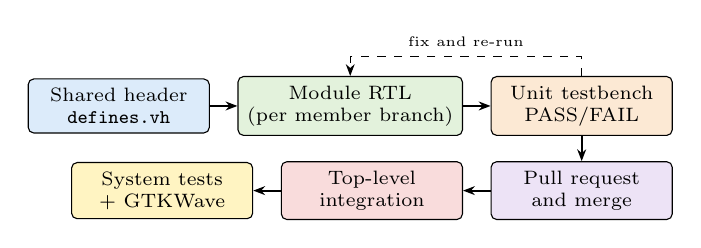
\begin{tikzpicture}[font=\scriptsize, >={Stealth[length=1.5mm]},
  st/.style={draw, rounded corners=2pt, fill=white, minimum width=2.3cm, minimum height=0.62cm, align=center},
  node distance=0.32cm and 0.35cm]
\node[st, fill=stIF]  (a) {Shared header\\\texttt{defines.vh}};
\node[st, fill=stID, right=of a] (b) {Module RTL\\(per member branch)};
\node[st, fill=stEX, right=of b] (c) {Unit testbench\\PASS/FAIL};
\node[st, fill=stMEM, below=of c] (d) {Pull request\\and merge};
\node[st, fill=stWB, left=of d] (e) {Top-level\\integration};
\node[st, fill=hz, left=of e] (f) {System tests\\+ GTKWave};
\draw[->, thick] (a) -- (b);
\draw[->, thick] (b) -- (c);
\draw[->, thick] (c) -- (d);
\draw[->, thick] (d) -- (e);
\draw[->, thick] (e) -- (f);
\draw[->, dashed] (c.north) -- ++(0,0.25) -| node[pos=0.25, above, font=\tiny]{fix and re-run} (b.north);
\end{tikzpicture}
\caption{Interface-first design and verification flow used by the team.}
\label{fig:flow}
\end{figure}

\begin{table}[!t]
\centering
\caption{Verilog Modules of the Processor}
\label{tab:modules}
\setlength{\tabcolsep}{3pt}
\renewcommand{\arraystretch}{1.05}
\begin{tabular}{@{}lll@{}}
\toprule
\textbf{Module} & \textbf{Stage} & \textbf{Function} \\ \midrule
\texttt{pc\_reg}          & IF  & program counter with enable \\
\texttt{instr\_mem}       & IF  & 1024-word instruction ROM \\
\texttt{if\_id\_reg}      & IF/ID & latch, hold, flush to NOP \\
\texttt{reg\_file}        & ID  & 32$\times$32 registers, write-first \\
\texttt{imm\_gen}         & ID  & I/S/B/U/J immediates \\
\texttt{control\_unit}    & ID  & opcode decoder \\
\texttt{id\_ex\_reg}      & ID/EX & latch, flush to bubble \\
\texttt{alu\_control}     & EX  & selects 1 of 10 ALU ops \\
\texttt{alu}              & EX  & arithmetic, logic, shifts, compare \\
\texttt{branch\_unit}     & EX  & branch decision and target \\
\texttt{ex\_stage}        & EX  & forwarding muxes + above three \\
\texttt{ex\_mem\_reg}     & EX/MEM & pipeline register \\
\texttt{data\_mem}        & MEM & 1024-word data RAM \\
\texttt{mem\_wb\_reg}     & MEM/WB & pipeline register \\
\texttt{forwarding\_unit} & EX  & selects operand sources \\
\texttt{hazard\_unit}     & ID  & stall and flush control \\
\texttt{riscv\_pipeline\_top} & -- & integration, PC and WB muxes \\ \bottomrule
\end{tabular}
\end{table}

\subsection{Instruction Fetch (IF)}
The \texttt{pc\_reg} module holds the program counter. It loads
\texttt{pc\_next} on each clock edge when its enable \texttt{pc\_write} is high and holds
its value during a stall. The next-PC multiplexer selects
\begin{equation}
pc_{next} = \begin{cases} branch\_target, & pc\_src = 1\\ pc + 4, & \text{otherwise.}\end{cases}
\end{equation}
The \texttt{instr\_mem} module loads a program from a hex file with
\texttt{\$readmemh} and returns the word at \texttt{addr[11:2]}; unused words are
initialised to the canonical NOP (\texttt{addi x0,x0,0}). The IF/ID register latches the
PC and instruction; on reset or flush it outputs a NOP, and when \texttt{if\_id\_write}
is low it holds its contents.

\subsection{Instruction Decode (ID)}
The \texttt{control\_unit} decodes the 7-bit opcode into the control signals of
Table~\ref{tab:ctrl}. The \texttt{imm\_gen} module sign-extends the I, S, B, U and J
immediate formats according to the opcode. The \texttt{reg\_file} has 32 registers with
two combinational read ports and one write port; \texttt{x0} always reads as zero.
It implements a \emph{write-first bypass}: when WB writes register \texttt{rd} in the same
cycle that ID reads it, the new value is returned directly, which removes the WB-to-ID
hazard without any extra forwarding path. The ID/EX register passes all control and data
signals forward; on reset or flush it outputs all zeros, which is a bubble (no register
or memory write).

\begin{table}[!t]
\centering
\caption{Main Control Unit Truth Table}
\label{tab:ctrl}
\setlength{\tabcolsep}{2.6pt}
\renewcommand{\arraystretch}{1.1}
\begin{tabular}{@{}lccccccc@{}}
\toprule
\textbf{Opcode} & \textbf{RegW} & \textbf{MemR} & \textbf{MemW} & \textbf{M2R} & \textbf{ALUSrc} & \textbf{ALUOp} & \textbf{Other} \\ \midrule
R-type & 1 & 0 & 0 & 0 & 0 & 10 & -- \\
I-type & 1 & 0 & 0 & 0 & 1 & 11 & -- \\
LW     & 1 & 1 & 0 & 1 & 1 & 00 & -- \\
SW     & 0 & 0 & 1 & 0 & 1 & 00 & -- \\
Branch & 0 & 0 & 0 & 0 & 0 & 01 & branch \\
JAL    & 1 & 0 & 0 & 0 & 0 & 00 & jump \\
JALR   & 1 & 0 & 0 & 0 & 1 & 00 & jalr \\
LUI    & 1 & 0 & 0 & 0 & 1 & 00 & lui \\ \bottomrule
\end{tabular}
\end{table}

\subsection{Execute (EX)}
The \texttt{ex\_stage} wrapper contains the operand forwarding multiplexers, the
\texttt{alu\_control}, the \texttt{alu} and the \texttt{branch\_unit}. The ALU control maps
\texttt{alu\_op}, \texttt{funct3} and bit~5 of \texttt{funct7} to one of ten ALU
operations (ADD, SUB, AND, OR, XOR, SLL, SRL, SRA, SLT, SLTU). Operand~A is the forwarded
\texttt{rs1} value, or zero for LUI so that the ALU computes $0 + imm$. Operand~B is the
forwarded \texttt{rs2} value or the immediate, selected by \texttt{alu\_src}. The value
stored by SW is the forwarded \texttt{rs2}, so a store directly after the producing
instruction still writes the correct data.

The branch unit compares the forwarded operands for BEQ, BNE, BLT and BGE (signed) and
computes the target: $pc + imm$ for branches and JAL, and $(rs1 + imm)\,\&\,\sim\!1$ for
JALR. It asserts \texttt{pc\_src} when a branch is taken or for any jump. For JAL and
JALR the stage result is the link address:
\begin{equation}
ex\_result = (jump \lor jalr)\ ?\ pc + 4 : alu\_out .
\end{equation}

\subsection{Memory (MEM) and Write-Back (WB)}
The \texttt{data\_mem} module writes \texttt{wdata} on the rising edge when
\texttt{mem\_write} is set and returns \texttt{mem[addr[11:2]]} combinationally when
\texttt{mem\_read} is set (zero otherwise). The MEM/WB register carries the ALU result,
the loaded data, \texttt{rd} and the two remaining control bits. In WB the result is
selected as
\begin{equation}
wb\_data = mem\_to\_reg\ ?\ wb\_mem\_rdata : wb\_result
\end{equation}
and written to the register file when \texttt{wb\_reg\_write} is set.

\subsection{Hazard Handling}

\subsubsection{Structural hazards}
Separate instruction and data memories let IF and MEM access memory in the same cycle,
and the register file is read in ID and written in WB through separate ports. No
structural hazard remains.

\subsubsection{Data hazards and forwarding}
The \texttt{forwarding\_unit} compares the source registers of the instruction in EX with
the destination registers of the two older instructions:
\begin{align}
F_A &= \begin{cases}
10, & RegW_{M} \land rd_{M}\neq 0 \land rd_{M} = rs1_{E}\\
01, & RegW_{W} \land rd_{W}\neq 0 \land rd_{W} = rs1_{E}\\
00, & \text{otherwise}
\end{cases}
\end{align}
and $F_B$ is defined in the same way with $rs2_E$. Subscripts $M$ and $W$ denote the
EX/MEM and MEM/WB registers. The EX/MEM case is checked first because it holds the most
recent value of the register. Register \texttt{x0} is never forwarded.

\subsubsection{Load-use stall}
A loaded value exists only at the end of MEM, so it cannot be forwarded to an instruction
that enters EX in the very next cycle. The \texttt{hazard\_unit} detects this case in ID:
\begin{equation}
load\_use = MemR_E \land rd_E \neq 0 \land (rd_E = rs1_D \lor rd_E = rs2_D).
\end{equation}
When it is true, \texttt{pc\_write} and \texttt{if\_id\_write} are cleared, so the PC and
IF/ID hold, and \texttt{id\_ex\_flush} inserts a bubble. In the next cycle the load is in
WB and its value is forwarded from MEM/WB. Fig.~\ref{fig:timing} and
Table~\ref{tab:loaduse} show this for the program
\texttt{lw x2,0(x0); add x3,x2,x2}. The table was taken from the simulation trace of
system test~4.

% ---------------- Pipeline timing figure ----------------
\begin{figure}[!t]
\centering
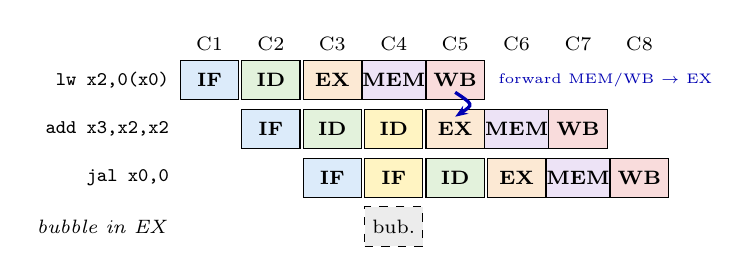
\begin{tikzpicture}[x=0.78cm, y=0.62cm, font=\scriptsize]
\tikzset{
  c/.style={draw, minimum width=0.74cm, minimum height=0.5cm, inner sep=0pt, font=\scriptsize\bfseries},
}
\foreach \i in {1,...,8} \node at (\i,0.75) {C\i};
\node[anchor=east] at (0.5,0) {\texttt{lw x2,0(x0)}};
\node[anchor=east] at (0.5,-1) {\texttt{add x3,x2,x2}};
\node[anchor=east] at (0.5,-2) {\texttt{jal x0,0}};
% lw
\node[c, fill=stIF]  at (1,0) {IF};
\node[c, fill=stID]  at (2,0) {ID};
\node[c, fill=stEX]  at (3,0) {EX};
\node[c, fill=stMEM] at (4,0) {MEM};
\node[c, fill=stWB]  at (5,0) {WB};
% add
\node[c, fill=stIF]  at (2,-1) {IF};
\node[c, fill=stID]  at (3,-1) {ID};
\node[c, fill=hz]    at (4,-1) {ID};
\node[c, fill=stEX]  at (5,-1) {EX};
\node[c, fill=stMEM] at (6,-1) {MEM};
\node[c, fill=stWB]  at (7,-1) {WB};
% jal
\node[c, fill=stIF]  at (3,-2) {IF};
\node[c, fill=hz]    at (4,-2) {IF};
\node[c, fill=stID]  at (5,-2) {ID};
\node[c, fill=stEX]  at (6,-2) {EX};
\node[c, fill=stMEM] at (7,-2) {MEM};
\node[c, fill=stWB]  at (8,-2) {WB};
% bubble
\node[c, dashed, fill=gray!15, font=\scriptsize] at (4,-3) {bub.};
\node[anchor=east] at (0.5,-3) {\textit{bubble in EX}};
% forwarding arrow
\draw[-{Stealth[length=1.6mm]}, very thick, blue!70!black] (5,-0.25) .. controls (5.3,-0.5) .. (5,-0.75);
\node[blue!70!black, anchor=west, font=\tiny] at (5.55,0) {forward MEM/WB $\rightarrow$ EX};
\end{tikzpicture}
\caption{Pipeline timing for a load-use dependency. The dependent \texttt{add} is held in
ID for one cycle (yellow) while a bubble enters EX; the loaded value is then forwarded from
MEM/WB.}
\label{fig:timing}
\end{figure}

\begin{table}[!t]
\centering
\caption{Simulated Hazard Signals for the Load-Use Example (Test 4)}
\label{tab:loaduse}
\setlength{\tabcolsep}{3pt}
\renewcommand{\arraystretch}{1.1}
\begin{tabular}{@{}cccccc@{}}
\toprule
\textbf{Cycle} & \textbf{PC} & \textbf{Instr. in ID} & \textbf{pc\_write} & \textbf{id\_ex\_flush} & $F_A/F_B$ \\ \midrule
4 & 0x0C & \texttt{lw x2}          & 1 & 0 & 00/10 \\
5 & 0x10 & \texttt{add x3,x2,x2}   & \textbf{0} & \textbf{1} & 00/00 \\
6 & 0x10 & \texttt{add x3,x2,x2}   & 1 & 0 & 00/00 \\
7 & 0x14 & \texttt{jal x0,0}       & 1 & 0 & \textbf{01/01} \\ \bottomrule
\end{tabular}
\end{table}

\subsubsection{Control hazards}
Branches and jumps are resolved in EX with a predict-not-taken policy. When
\texttt{pc\_src} is asserted, the two younger instructions in IF/ID and ID/EX are on the
wrong path, so the hazard unit sets \texttt{if\_id\_flush} and \texttt{id\_ex\_flush}
and loads the target into the PC. A taken branch therefore costs two cycles; a not-taken
branch costs nothing. Flush has priority over a simultaneous load-use stall, because the
stalled instruction is itself on the wrong path. The complete hazard unit is:
\begin{center}
\footnotesize\setlength{\tabcolsep}{3pt}
\begin{tabular}{@{}lcccc@{}}
\toprule
\textbf{Condition} & \textbf{pc\_write} & \textbf{if\_id\_write} & \textbf{if\_id\_flush} & \textbf{id\_ex\_flush} \\ \midrule
\texttt{pc\_src}          & 1 & 1 & 1 & 1 \\
\texttt{load\_use} only   & 0 & 0 & 0 & 1 \\
neither                   & 1 & 1 & 0 & 0 \\ \bottomrule
\end{tabular}
\end{center}
Fig.~\ref{fig:hazflow} shows the same decision order as a flowchart.
\begin{figure}[!t]
\centering
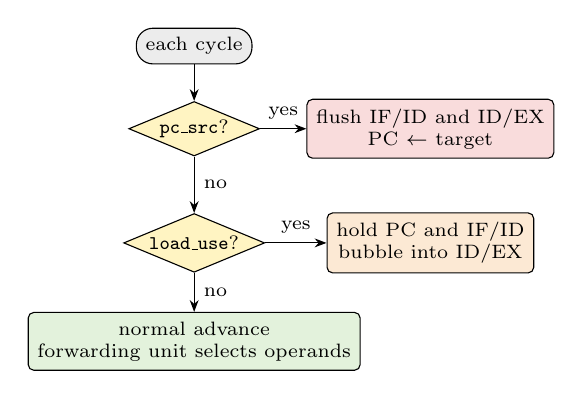
\begin{tikzpicture}[font=\scriptsize, >={Stealth[length=1.5mm]},
  dec/.style={draw, diamond, aspect=2.4, fill=hz, inner sep=1pt, align=center},
  act/.style={draw, rounded corners=2pt, fill=white, align=center, minimum width=2.6cm, minimum height=0.55cm}]
\node[draw, rounded corners=6pt, fill=gray!15] (s) at (0,0) {each cycle};
\node[dec] (d1) at (0,-1.05) {\texttt{pc\_src}?};
\node[act, fill=stWB] (a1) at (3.0,-1.05) {flush IF/ID and ID/EX\\PC $\leftarrow$ target};
\node[dec] (d2) at (0,-2.5) {\texttt{load\_use}?};
\node[act, fill=stEX] (a2) at (3.0,-2.5) {hold PC and IF/ID\\bubble into ID/EX};
\node[act, fill=stID] (a3) at (0,-3.75) {normal advance\\forwarding unit selects operands};
\draw[->] (s) -- (d1);
\draw[->] (d1) -- node[above]{yes} (a1);
\draw[->] (d1) -- node[right]{no} (d2);
\draw[->] (d2) -- node[above]{yes} (a2);
\draw[->] (d2) -- node[right]{no} (a3);
\end{tikzpicture}
\caption{Decision order of the hazard detection unit. A taken branch or jump is checked
first, so flushing always overrides a load-use stall.}
\label{fig:hazflow}
\end{figure}

Fig.~\ref{fig:flush} shows the flush observed for \texttt{beq x1,x2,8} in system test~5:
the branch is taken in cycle~5 and the instructions at 0x0C and 0x10 are discarded.

\begin{figure}[!t]
\centering
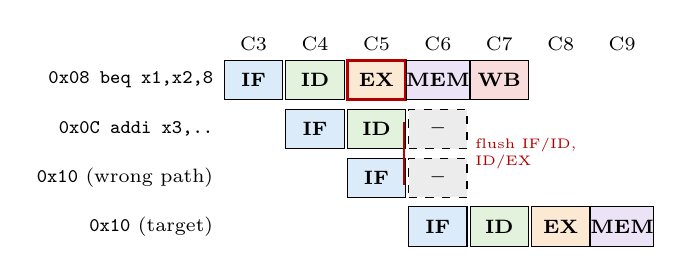
\begin{tikzpicture}[x=0.78cm, y=0.62cm, font=\scriptsize]
\tikzset{c/.style={draw, minimum width=0.74cm, minimum height=0.5cm, inner sep=0pt, font=\scriptsize\bfseries}}
\foreach \i in {3,...,9} \node at (\i-2,0.75) {C\i};
\node[anchor=east] at (0.5,0)  {\texttt{0x08 beq x1,x2,8}};
\node[anchor=east] at (0.5,-1) {\texttt{0x0C addi x3,..}};
\node[anchor=east] at (0.5,-2) {\texttt{0x10} (wrong path)};
\node[anchor=east] at (0.5,-3) {\texttt{0x10} (target)};
\node[c, fill=stIF] at (1,0) {IF};
\node[c, fill=stID] at (2,0) {ID};
\node[c, fill=stEX, line width=1.2pt, draw=red!70!black] at (3,0) {EX};
\node[c, fill=stMEM] at (4,0) {MEM};
\node[c, fill=stWB] at (5,0) {WB};
\node[c, fill=stIF] at (2,-1) {IF};
\node[c, fill=stID] at (3,-1) {ID};
\node[c, dashed, fill=gray!15] at (4,-1) {--};
\node[c, fill=stIF] at (3,-2) {IF};
\node[c, dashed, fill=gray!15] at (4,-2) {--};
\node[c, fill=stIF] at (4,-3) {IF};
\node[c, fill=stID] at (5,-3) {ID};
\node[c, fill=stEX] at (6,-3) {EX};
\node[c, fill=stMEM] at (7,-3) {MEM};
\draw[red!70!black, thick] (3.45,-0.85) -- (3.45,-2.15);
\node[red!70!black, anchor=west, font=\tiny, align=left] at (4.45,-1.5) {flush IF/ID,\\ ID/EX};
\end{tikzpicture}
\caption{Branch resolution in EX (cycle 5) and flushing of the two wrongly fetched
instructions, as observed in system test 5. The taken branch costs two cycles.}
\label{fig:flush}
\end{figure}

\subsection{Implementation and Tools}
The design consists of 17 Verilog modules sharing one header (\texttt{defines.vh}) for
opcodes, ALU control codes and the NOP encoding~\cite{ieee1364}. Port names follow a
fixed rule: a pipeline-register input carries its source-stage prefix and the matching
output carries the destination-stage prefix (for example \texttt{ex\_result} to
\texttt{mem\_result}). The top module \texttt{riscv\_pipeline\_top} instantiates and wires
all modules and contains the PC and write-back multiplexers. Simulation uses Icarus
Verilog~\cite{iverilog} and waveforms are viewed in GTKWave~\cite{gtkwave}. Source code is
version-controlled on GitHub, with each member working on a separate branch merged through
pull requests.

% ---------------------------------------------------------------------------
\section{Verification and Performance}
Every module has a self-checking unit testbench that applies directed stimulus, prints
PASS or FAIL for each check and dumps a VCD waveform. Six assembly programs exercise the
full pipeline; the system testbench runs each program for 300 cycles and then checks
register and data-memory contents. A single script, \texttt{simulation/run\_all.sh}, runs
the whole suite. Table~\ref{tab:tests} summarises the results; all checks pass.

During system testing four testbench-side defects were found and fixed: the hex image
of test~1 had lost one instruction and encoded SRAI as SRLI, the hex encoding of three
branch instructions in test~5 did not match its assembly source, the
final \texttt{jalr} of test~5 looped back instead of reaching the halt instruction, and
the VCD file-name buffer in the system testbench was too short for the output path. None
of them required a change to the processor RTL.

\begin{table}[!t]
\centering
\caption{Verification Results (Icarus Verilog 13.0)}
\label{tab:tests}
\setlength{\tabcolsep}{3pt}
\renewcommand{\arraystretch}{1.08}
\begin{tabular}{@{}>{\raggedright\arraybackslash}p{5.0cm}cc@{}}
\toprule
\textbf{Testbench / Program} & \textbf{Checks} & \textbf{Result} \\ \midrule
\multicolumn{3}{@{}l}{\textit{Unit testbenches}} \\
\texttt{pc\_reg}, \texttt{instr\_mem}, \texttt{if\_id\_reg} & 21 & PASS \\
\texttt{reg\_file}, \texttt{imm\_gen}, \texttt{control\_unit}, \texttt{id\_ex\_reg} & 53 & PASS \\
\texttt{alu}, \texttt{alu\_control}, \texttt{branch\_unit}, \texttt{ex\_stage}, \texttt{ex\_mem\_reg} & 101 & PASS \\
\texttt{data\_mem}, \texttt{mem\_wb\_reg}, \texttt{forwarding\_unit}, \texttt{hazard\_unit} & 29 & PASS \\ \midrule
\multicolumn{3}{@{}l}{\textit{System programs}} \\
1: arithmetic, logic, LUI & 18 & PASS \\
2: load / store & 4 & PASS \\
3: back-to-back forwarding & 3 & PASS \\
4: load-use stall & 3 & PASS \\
5: branches, JAL, JALR, flush & 6 & PASS \\
6: array-sum loop & 2 & PASS \\ \midrule
\textbf{Total} & \textbf{240} & \textbf{PASS} \\ \bottomrule
\end{tabular}
\end{table}


Table~\ref{tab:programs} describes the six system programs. Each is written in RISC-V
assembly (\texttt{.s}) and hand-assembled into a hex image loaded by the instruction
memory. Every program ends with \texttt{jal x0,0}, an infinite loop that keeps the
pipeline in a known state until the checks run.

\begin{table}[!t]
\centering
\caption{System Test Programs}
\label{tab:programs}
\setlength{\tabcolsep}{3pt}
\renewcommand{\arraystretch}{1.08}
\begin{tabular}{@{}>{\raggedright\arraybackslash}p{1.6cm}>{\raggedright\arraybackslash}p{3.7cm}>{\raggedright\arraybackslash}p{2.3cm}@{}}
\toprule
\textbf{Program} & \textbf{Exercises} & \textbf{Checked state} \\ \midrule
1 arith    & LUI and all R-type and I-type ALU operations & x1, x4--x20 \\
2 loadstore & SW then LW of two words     & mem[0], mem[1], x3, x4 \\
3 forwarding & back-to-back dependent ADD/ADDI (EX/MEM and MEM/WB paths) & x3, x4, x5 \\
4 loaduse  & LW followed by a dependent ADD & mem[0], x2, x3 \\
5 branch\_jump & taken BEQ, not-taken BLT, JAL, JALR, flushed instructions & x3, x5--x9 \\
6 sum\_array & loop with loads, branch and store & word at byte 20, x8 \\ \bottomrule
\end{tabular}
\end{table}

Fig.~\ref{fig:wave} redraws the key signals of test~4 as a timing diagram. The values were
read from the simulation trace one nanosecond after each rising edge. The stall is visible
in cycle~5: \texttt{pc\_write} drops, the PC stays at \texttt{0x10} for two cycles and
\texttt{id\_ex\_flush} inserts the bubble. In cycle~7 both forwarding selects are
\texttt{01}, so \texttt{add x3,x2,x2} takes the loaded value from MEM/WB. In cycle~8 the
final \texttt{jal x0,0} is taken, \texttt{pc\_src} rises and both flush signals fire.

\begin{figure}[!t]
\centering
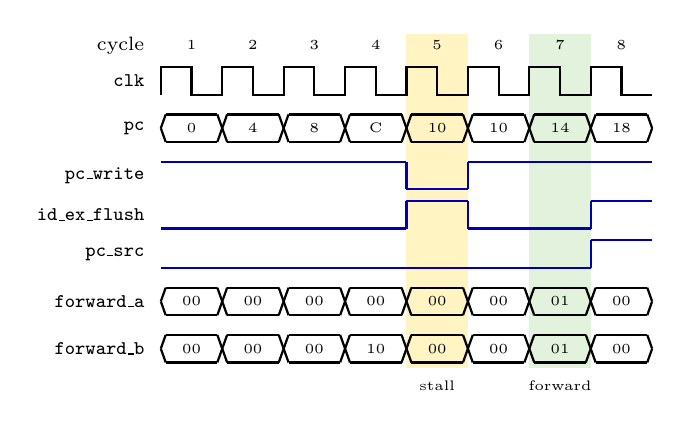
\begin{tikzpicture}[x=0.78cm, y=0.5cm, font=\tiny, thick]
\def\lab#1#2{\node[anchor=east, font=\scriptsize] at (-0.1,#1) {#2};}
\fill[hz] (4,1.2) rectangle (5,-7.3);
\node[font=\tiny] at (4.5,-7.75) {stall};
\fill[stID] (6,1.2) rectangle (7,-7.3);
\node[font=\tiny] at (6.5,-7.75) {forward};
\foreach \i in {1,...,8} \node[font=\tiny] at (\i-0.5,0.9) {\i};
\node[anchor=east, font=\scriptsize] at (-0.1,0.9) {cycle};
% clock
\lab{0}{\texttt{clk}}
\draw (0,-0.35) \foreach \i in {0,...,7} { -- (\i,0.35) -- (\i+0.5,0.35) -- (\i+0.5,-0.35) -- (\i+1,-0.35)};
% PC bus
\lab{-1.2}{\texttt{pc}}
\foreach \i/\v in {0/0,1/4,2/8,3/C,4/10,5/10,6/14,7/18} {
  \draw (\i+0.08,-0.85) -- (\i+0.92,-0.85); \draw (\i+0.08,-1.55) -- (\i+0.92,-1.55);
  \draw (\i,-1.2) -- (\i+0.08,-0.85); \draw (\i,-1.2) -- (\i+0.08,-1.55);
  \draw (\i+1,-1.2) -- (\i+0.92,-0.85); \draw (\i+1,-1.2) -- (\i+0.92,-1.55);
  \node at (\i+0.5,-1.2) {\v};}
% single-bit signals: name, y, values
\foreach \nm/\y/\vals in {pc\_write/-2.4/{1,1,1,1,0,1,1,1}, id\_ex\_flush/-3.4/{0,0,0,0,1,0,0,1}, pc\_src/-4.4/{0,0,0,0,0,0,0,1}} {
  \node[anchor=east, font=\scriptsize] at (-0.1,\y) {\texttt{\nm}};
  \foreach [count=\k from 0] \b in \vals {
    \pgfmathsetmacro{\yy}{\y+(\b-0.5)*0.7}
    \draw[blue!70!black] (\k,\yy) -- (\k+1,\yy);
  }
}
\draw[blue!70!black] (4,-2.05) -- (4,-2.75); \draw[blue!70!black] (5,-2.05) -- (5,-2.75);
\draw[blue!70!black] (4,-3.05) -- (4,-3.75); \draw[blue!70!black] (5,-3.05) -- (5,-3.75);
\draw[blue!70!black] (7,-3.05) -- (7,-3.75); \draw[blue!70!black] (7,-4.05) -- (7,-4.75);
% forwarding selects
\foreach \nm/\y/\vals in {forward\_a/-5.6/{00,00,00,00,00,00,01,00}, forward\_b/-6.8/{00,00,00,10,00,00,01,00}} {
  \node[anchor=east, font=\scriptsize] at (-0.1,\y) {\texttt{\nm}};
  \foreach [count=\k from 0] \v in \vals {
    \draw (\k+0.08,\y+0.35) -- (\k+0.92,\y+0.35); \draw (\k+0.08,\y-0.35) -- (\k+0.92,\y-0.35);
    \draw (\k,\y) -- (\k+0.08,\y+0.35); \draw (\k,\y) -- (\k+0.08,\y-0.35);
    \draw (\k+1,\y) -- (\k+0.92,\y+0.35); \draw (\k+1,\y) -- (\k+0.92,\y-0.35);
    \node at (\k+0.5,\y) {\v};}
}
\end{tikzpicture}
\caption{Timing diagram of system test 4 drawn from the simulation trace (PC in hex).
Shaded columns mark the load-use stall (cycle 5) and the MEM/WB forwarding (cycle 7).}
\label{fig:wave}
\end{figure}

\subsection{Performance: Measured CPI}
The system testbench contains a small performance counter that does not change the
design. It tracks a valid bit for IF/ID, counts an instruction when it leaves ID for EX,
and stops when the final \texttt{jal x0,0} leaves ID. That instruction completes WB three
cycles later, which gives the total cycle count $C$. With $N$ executed instructions, $S$
load-use stall cycles and $T$ taken branches or jumps (before the halt), the five-stage
pipeline should need
\begin{equation}
C = N + 4 + S + 2T
\end{equation}
cycles: four cycles to fill the pipeline, one extra cycle per stall and two per taken
transfer. Table~\ref{tab:cpi} shows that every measured count matches this model exactly.
$\mathrm{CPI} = C/N$ and $\mathrm{IPC} = N/C$.

\begin{table}[!t]
\centering
\caption{Measured Cycles and CPI (Icarus Verilog Simulation)}
\label{tab:cpi}
\setlength{\tabcolsep}{4pt}
\renewcommand{\arraystretch}{1.08}
\begin{tabular}{@{}lcccccc@{}}
\toprule
\textbf{Program} & $N$ & $S$ & $T$ & $C$ & \textbf{CPI} & \textbf{IPC} \\ \midrule
1 arith       & 21 & 0 & 0 & 25 & 1.19 & 0.84 \\
2 loadstore   & 7  & 0 & 0 & 11 & 1.57 & 0.64 \\
3 forwarding  & 6  & 0 & 0 & 10 & 1.67 & 0.60 \\
4 loaduse     & 5  & 1 & 0 & 10 & 2.00 & 0.50 \\
5 branch\_jump & 11 & 0 & 4 & 23 & 2.09 & 0.48 \\
6 sum\_array  & 40 & 5 & 4 & 57 & 1.43 & 0.70 \\ \bottomrule
\end{tabular}
\end{table}

The programs are short, so the four fill cycles dominate their CPI. Test~3 shows the
value of forwarding: three back-to-back dependent instructions add no cycles at all.
Without forwarding, each would have to wait until its producer wrote the register file.
Test~6, a five-iteration loop, has the most realistic mix. Its five load-use stalls and
four taken \texttt{bne} branches cost 13 of its 57 cycles.

As a baseline, consider a non-pipelined (multicycle) design with the same stages and the
same clock period, which needs five cycles for every instruction, i.e.\ $5N$ cycles.
Fig.~\ref{fig:cycles} compares it with the measured pipeline. On test~6 the pipeline
needs 57 cycles instead of 200, a speed-up of $200/57 \approx 3.5\times$, below the ideal
$5\times$ because of fill, stall and flush cycles. A single-cycle design has CPI~$=1$ but
a clock period about as long as all five stages together, so its execution time is close
to the multicycle baseline. Synthesis results (resource use and maximum clock frequency),
which would convert these cycle counts into time, are planned for Phase~II.

\begin{figure}[!t]
\centering
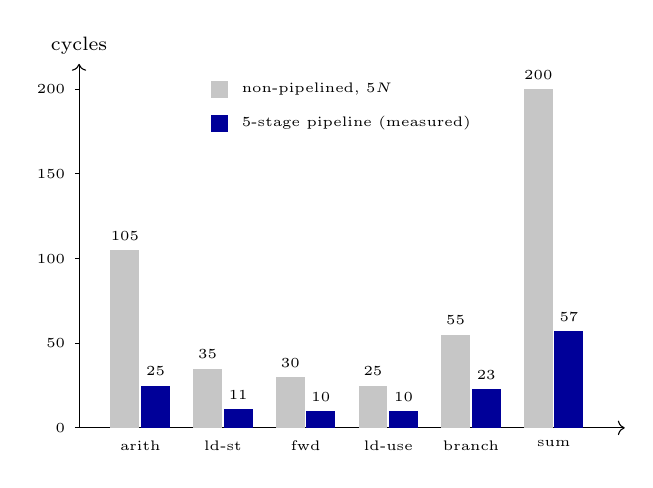
\begin{tikzpicture}[x=1.05cm, y=0.0215cm, font=\scriptsize]
\draw[->] (0,0) -- (6.6,0);
\draw[->] (0,0) -- (0,215) node[above, font=\scriptsize] {cycles};
\foreach \v in {0,50,100,150,200} {\draw (-0.05,\v) -- (0,\v); \node[anchor=east, font=\tiny] at (-0.05,\v) {\v};}
\foreach \i/\n/\c/\name in {1/21/25/arith, 2/7/11/ld-st, 3/6/10/fwd, 4/5/10/ld-use, 5/11/23/branch, 6/40/57/sum} {
  \pgfmathtruncatemacro{\b}{5*\n}
  \fill[gray!45] (\i-0.62,0) rectangle (\i-0.27,\b);
  \fill[blue!60!black] (\i-0.25,0) rectangle (\i+0.1,\c);
  \node[font=\tiny, anchor=south] at (\i-0.445,\b) {\b};
  \node[font=\tiny, anchor=south] at (\i-0.075,\c) {\c};
  \node[font=\tiny, anchor=north] at (\i-0.26,-2) {\name};
}
\fill[gray!45] (1.6,195) rectangle (1.8,205); \node[anchor=west, font=\tiny] at (1.85,200) {non-pipelined, $5N$};
\fill[blue!60!black] (1.6,175) rectangle (1.8,185); \node[anchor=west, font=\tiny] at (1.85,180) {5-stage pipeline (measured)};
\end{tikzpicture}
\caption{Total cycles per test program: measured five-stage pipeline versus a
non-pipelined baseline that needs five cycles per instruction at the same clock period.}
\label{fig:cycles}
\end{figure}

\subsection*{Demonstration Video}
A demonstration video introducing the team, the design and the simulation results is
available at \url{https://drive.google.com/drive/folders/1MsBRF6YmyPTbTrJbZ43O3noa1C6fjQQy?usp=sharing}.

\subsection*{Limitations and Phase II Plan}
The design supports only word loads and stores, a subset of branches, and no CSR,
exception or interrupt handling. Branches use static not-taken prediction, so every taken
branch costs two cycles. The hazard unit also compares the \texttt{rs2} field for every
instruction, so an I-type instruction whose immediate bits happen to match a load's
destination can stall one unnecessary cycle; this is safe but slightly conservative.
Phase~II will add synthesis results, larger benchmark programs and a fuller performance
discussion.

% ---------------------------------------------------------------------------
\section{Individual Contributions}

\textbf{Abhishek Kumar Patel (2401010020)} -- Project lead. Set up the GitHub repository
and branch workflow, wrote the shared header \texttt{defines.vh}, fixed the port list of every
module, and designed the IF stage
(\texttt{pc\_reg}, \texttt{instr\_mem}, \texttt{if\_id\_reg}) with its unit testbenches.
Integrated all modules in \texttt{riscv\_pipeline\_top}, including the PC and write-back
multiplexers, and assembled this report.

\textbf{Yogesh Modi (2401010519)} -- Designed the ID stage: the register file with
write-first bypass, the immediate generator for all five formats, the main control unit
and the ID/EX pipeline register, each with a unit testbench. Wrote the literature review.

\textbf{Kapish Rohilla (2401010210)} -- Designed the EX stage: the ten-operation ALU, the
ALU control decoder, the branch unit for BEQ/BNE/BLT/BGE/JAL/JALR, the EX-stage wrapper
with operand-forwarding multiplexers and link-address selection, and the EX/MEM pipeline
register, each with a unit testbench.

\textbf{Vikash Kumar (2401010503)} -- Designed the MEM and WB stages and the hazard logic:
the data memory, the MEM/WB pipeline register, the forwarding unit and the hazard
detection unit for load-use stalls and branch flushes, each with a unit testbench.

\textbf{Prateek Shakya (2401020048)} -- Built the verification environment: the system
testbench, the six assembly test programs with their hex images, and the
\texttt{run\_all.sh} script. Prepared the datapath, hazard and pipeline-timing diagram
sketches and the demonstration video.

% ---------------------------------------------------------------------------
\begin{thebibliography}{99}
\bibitem{rvmanual}
A.~Waterman and K.~Asanovi\'c, Eds., \emph{The RISC-V Instruction Set Manual, Volume I:
Unprivileged ISA}, Document Version 20191213, RISC-V Foundation, Dec. 2019.

\bibitem{waterman2011}
A.~Waterman, Y.~Lee, D.~A. Patterson, and K.~Asanovi\'c, ``The RISC-V instruction set
manual, Volume I: Base user-level ISA,'' EECS Dept., Univ. of California, Berkeley,
Tech. Rep. UCB/EECS-2011-62, May 2011.

\bibitem{asanovic2014free}
K.~Asanovi\'c and D.~A. Patterson, ``Instruction sets should be free: The case for
RISC-V,'' EECS Dept., Univ. of California, Berkeley, Tech. Rep. UCB/EECS-2014-146,
Aug. 2014.

\bibitem{pattersonRV}
D.~A. Patterson and J.~L. Hennessy, \emph{Computer Organization and Design RISC-V
Edition: The Hardware/Software Interface}, 2nd~ed. Cambridge, MA, USA: Morgan Kaufmann,
2020.

\bibitem{hennessyQA}
J.~L. Hennessy and D.~A. Patterson, \emph{Computer Architecture: A Quantitative
Approach}, 6th~ed. Cambridge, MA, USA: Morgan Kaufmann, 2017.

\bibitem{harrisRV}
S.~L. Harris and D.~M. Harris, \emph{Digital Design and Computer Architecture: RISC-V
Edition}. Cambridge, MA, USA: Morgan Kaufmann, 2021.

\bibitem{patterson1980risc}
D.~A. Patterson and D.~R. Ditzel, ``The case for the reduced instruction set computer,''
\emph{ACM SIGARCH Comput. Archit. News}, vol.~8, no.~6, pp.~25--33, Oct. 1980.

\bibitem{hennessy1982mips}
J.~Hennessy, N.~Jouppi, S.~Przybylski, C.~Rowen, T.~Gross, F.~Baskett, and J.~Gill,
``MIPS: A microprocessor architecture,'' in \emph{Proc. 15th Annu. Workshop
Microprogramming (MICRO-15)}, 1982, pp.~17--22.

\bibitem{tomasulo1967}
R.~M. Tomasulo, ``An efficient algorithm for exploiting multiple arithmetic units,''
\emph{IBM J. Res. Develop.}, vol.~11, no.~1, pp.~25--33, Jan. 1967.

\bibitem{rocket2016}
K.~Asanovi\'c \emph{et al.}, ``The Rocket Chip generator,'' EECS Dept., Univ. of
California, Berkeley, Tech. Rep. UCB/EECS-2016-17, Apr. 2016.

\bibitem{boom2015}
C.~Celio, D.~A. Patterson, and K.~Asanovi\'c, ``The Berkeley Out-of-Order Machine
(BOOM): An industry-competitive, synthesizable, parameterized RISC-V processor,'' EECS
Dept., Univ. of California, Berkeley, Tech. Rep. UCB/EECS-2015-167, Jun. 2015.

\bibitem{protocolx}
N.~Dhaterwal, ``protocolx-riscv-pipelined-processor,'' GitHub repository. [Online].
Available: \url{https://github.com/naveendhaterwal/protocolx-riscv-pipelined-processor}

\bibitem{ieee1364}
\emph{IEEE Standard for Verilog Hardware Description Language}, IEEE Std 1364-2005, 2006.

\bibitem{iverilog}
S.~Williams, ``Icarus Verilog.'' [Online]. Available:
\url{https://steveicarus.github.io/iverilog/}

\bibitem{gtkwave}
T.~Bybell, ``GTKWave.'' [Online]. Available: \url{https://gtkwave.sourceforge.net/}
\end{thebibliography}

\end{document}
